\begin{enumerate}[label=\thesection.\arabic*.,ref=\thesection.\theenumi]
\numberwithin{equation}{enumi}
\item The number of directions and encirclements around the point -1+j0 in the complex plane by the Nyquist plot of $G(s) = \frac{1-s}{4+2s}$\\

\solution
Substitute s = $\j\omega$ evaluate magnitude and phase from $\omega = -\infty$ to $\omega = \infty$
\begin{align}
G\brak{\j\omega} &= \frac{1-\j\omega}{4+2\j\omega} 
\end{align}

\item Phase of G\brak{\j\omega}
\begin{align}
\angle G\brak{\j\omega} = \angle G\brak{\j\omega}_{num} - \angle G\brak{\j\omega}_{den}
\end{align}
\begin{align}
\angle G\brak{\j\omega} &= \tan^{-1}\brak{\frac{-\omega}{1}} - \tan^{-1}\brak{\frac{\omega}{2}}
\end{align}
At $\omega = 0$ 
\begin{multline}
\angle G\brak{\j\omega} = \tan^{-1}\brak{0} - \tan^{-1}\brak{0} = 0
\end{multline}
At $\omega = \infty$ 
\begin{multline}
\angle G\brak{\j\omega} = \tan^{-1}\brak{-\infty} - \tan^{-1}\brak{\infty} = -180
\end{multline}
At $\omega = -\infty$ 
\begin{multline}
\angle G\brak{\j\omega} = \tan^{-1}\brak{\infty} - \tan^{-1}\brak{-\infty} = 180
\end{multline}

\item Magnitude of G\brak{\j\omega}
\begin{align}
\abs{G\brak{\j\omega}} &= \frac{\sqrt{1+{\omega}^2}}{\sqrt{16+{4\omega}^2}} 
\end{align}
At $\omega = 0$ 
\begin{align}
    \abs{G\brak{\j\omega}} &= \frac{1}{4}
\end{align}
At $\omega = \infty$ 
\begin{align}
    \abs{G\brak{\j\omega}} &= \frac{1}{2}
\end{align}
At $\omega = -\infty$ 
\begin{align}
    \abs{G\brak{\j\omega}} &= \frac{1}{2}
\end{align}

\item Nyquist plotting\\
\solution

From $\omega = 0$ to $\omega = \infty$ the path is
$\frac{1}{4}\angle0$ to $\frac{1}{2}\angle-180$
\\
From $\omega = -\infty$ to $\omega = 0$ the path is
$\frac{1}{2}\angle180$ to $\frac{1}{4}\angle0$

Substitute $s = Re^{\j\theta}$
\begin{align}
\lim_{R\to \infty}\,G\brak{Re^{\j\theta}} &= \frac{1-Re^{\j\theta}}{4+2Re^{\j\theta}}=\frac{-1}{2}  
\end{align}
As there are no $e^{\j\theta}$ terms.
There will be no enclosed Nyquist path here.
The Nyquist plot is the the Polar plot drawn by varying $\omega$ from $-\infty$ to $\infty$.

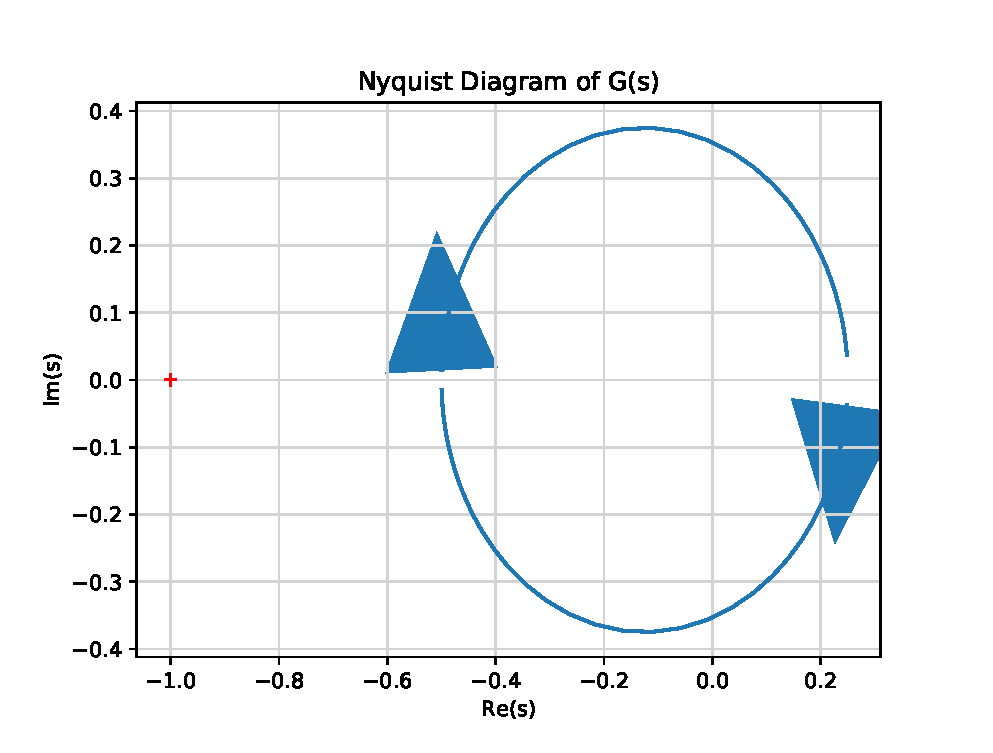
\includegraphics[width=\columnwidth]{./figs/ee18btech11034.eps}

Hence,the number of encirclements of -1+j0 is zero.\\
\begin{lstlisting}
codes/ee18btech11034.py
\end{lstlisting}
\end{enumerate}
